% fig_always.tex -- the two always-block recipes side by side
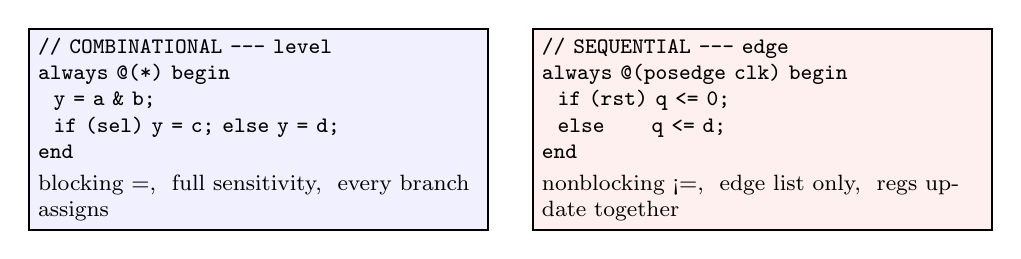
\begin{tikzpicture}[font=\small]
  \node[draw, thick, fill=blue!6, text width=5.6cm, align=left,
        font=\ttfamily\footnotesize, anchor=north west] at (0,0)
    {// COMBINATIONAL --- level\\
     always @(*) begin\\
     \ \ y = a \& b;\\
     \ \ if (sel) y = c; else y = d;\\
     end\\[2pt]
     \textrm{\footnotesize blocking =,\ \ full sensitivity,\ \ every branch assigns}};
  \node[draw, thick, fill=red!6, text width=5.6cm, align=left,
        font=\ttfamily\footnotesize, anchor=north west] at (6.4,0)
    {// SEQUENTIAL --- edge\\
     always @(posedge clk) begin\\
     \ \ if (rst) q <= 0;\\
     \ \ else\ \ \ \ \ \ q <= d;\\
     end\\[2pt]
     \textrm{\footnotesize nonblocking <=,\ \ edge list only,\ \ regs update together}};
\end{tikzpicture}
